%%%%%%%%%%%%%%%%%%%%%%%%%%%%%%%%%%%%%%%%%%%%%%%%%%%%%%%%%%%%%%%
%
% F1000Research is an open access publishing platform, with rapid publication times and an open and transparent peer review process. This template is for Software Tool articles, which should include the rationale for the development of the tool and details of the code used for its construction. The article should provide examples of suitable input data sets and include an example of the output that can be expected from the tool and how this output should be interpreted.
%
%%%%%%%%%%%%%%%%%%%%%%%%%%%%%%%%%%%%%%%%%%%%%%%%%%%%%%%%%%%%%%%
%
% For more detailed article preparation guidelines, please see:
% https://f1000research.com/for-authors/article-guidelines/software-tool-articles
%
% For more information on the F1000Research publishing model please see:
% https://f1000research.com/about

\documentclass[10pt,a4paper]{article}
\usepackage{f1000_styles}

%% Default: numerical citations
\usepackage[numbers]{natbib}

%% Uncomment this lines for superscript citations instead
% \usepackage[super]{natbib}

%% Uncomment these lines for author-year citations instead
% \usepackage[round]{natbib}
% \let\cite\citep

\begin{document}
\pagestyle{fancy}

\title{MotionRender: A simple Python implementation of video motion visualization for 3D motion capture data}
\author[1]{Derek Harter}
\author[2]{Shulan Lu}
\affil[1]{Derek.Harter@tamuc.edu, Department of Computer Science and Information Systems, Texas A\&M University - Commerce, Commerce, TX, 75428, USA}
\affil[2]{Shulan.Lu@tamuc.edu, Department of Psychology and Special Education, Texas A\&M University - Commerce, Commerce, TX, 75428, USA}

\maketitle
\thispagestyle{fancy}

\phantom{abstract is indented if this text is missing}
\\
\begin{abstract}

We describe a Python library project for generating animations of
simple 3D motion capture data points.  The motion capture method is
agnostic with respect to this visualizaiton tool, expecting a time
series of time stamped coordinates captured in a 3-dimensional space.
One of the advantages of this tool is the simple data format design.
This tool was developed originally for a Kinect system implementing
skeleton tracking of 15 joint positions, where each data point
consists of an accurate time of capture (time stamp), and 3 accurate
coordinate (x, y, z) positions of each of the 15 joints at each time
step.  In addition to the motion capture time series, all thaqt is
needed is a joint graph file describing the relationship of the joint
edges to one another.  This library can be extended to visualize and
create animations of motion capture data that can be reformulated
using this basic structure of a time series of time stamped 3D
coordinates and a joint graph description file.  This library should
be useful as is, or with easy modification, for many such
visualization requirements of similar motion capture data.
  

\end{abstract}

\section*{\color{f1ROrange}Keywords}

motion tracking, skeleton tracking, scientific visualization

\clearpage
\pagestyle{fancy}
\section*{Introduction}

Motion capture devices range from simple comsumer grade devices, like
the Kinect camera-based depth sensors \cite{pfister-2014, napoli-2017}
to more serious motion capture systems \cite{bregler-2007,menolotto-2020}
with fine spatial and fast temporal resolutions used
for generating mocap video rendering.
\\

Creating animated visualization in the base Python 3.X scientific
python stack is certainly much simpler than it has been in the past,
but still requires many specialized steps to achieve the task of
creating an animation that can be saved as a movie for presentation.
The standard Matplotlib animation library documentation
\cite{matplotlib-animation-2022} contains several examples of
generated animations, but only 1 of animating a 3D set of data
\cite{matplotlib-3d-random-walk-2022}.  The basic technique to use an
instance of \verb|matplotlib.animation| to generate a sequence of frames
from a set of 3D points is clear from the documentation, but can
certainly be difficult to generalize for much more complex data than
showing the basic example.
\\

3D motion capture data are a very useful type of data that needs to be
visualized to analyze its significance.  The goal of the
\verb|Motionrender| library is to simplify the task of creating
animated visualizations of such 3D time series data.  The library
presented here can be generalized to work with a time series of N 3D
points in space to create an animation of subsequent frames of the
captured points evolving over time.  The only additional general
information needed is a matrix of the relationship of the N points in
space that should be connected as being related points in the
resulting animation, known as a joint graph or joint edge graph
by the library.
\\

We used motion capture from a very basic Kinect skeleton tracking
experiment, using the NiTE 2.0 library \cite{nite-2.0-2022,
  nuitrack-2022} which includes skeleton tracking capture in the
development of this visualizaiton library.  However the general
format, described in methods, can be extended to many kinds of motion
capture devices where a timestamp and a set of 3D point positions can
be obtained for the captured object in motion.  In the example
implementation discussed, we have $N = 15$ joint positions (e.g. head,
neck, left shoulder, etc.) captured by the motion Kinect depth sensing
cameras.  An example of a rendered frame of the motion capture
animation is shown in Figure \ref{fig:rendered-joint-positions}.
Sample videos of the resulting animation are available in the
repository for this project, referenced below.
\\

\begin{figure}
	\centering
	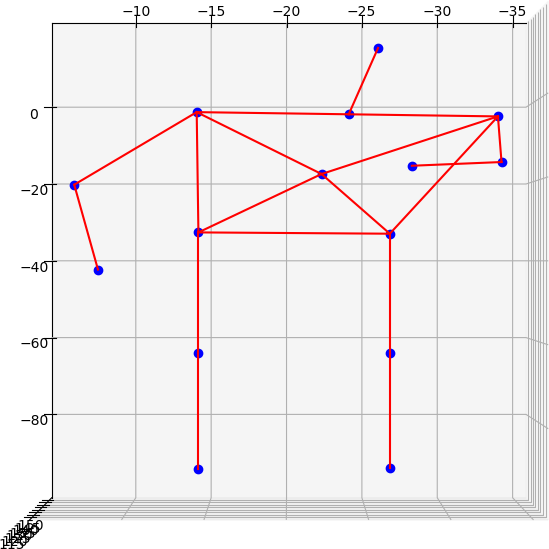
\includegraphics[width=0.66\textwidth]{rendered-joint-positions.png}
	\caption{\label{fig:rendered-joint-positions}[Example of a rendered frame of 3D motion capture joint positions}
\end{figure}


\section*{Methods}
\subsection*{Implementation}
The version of the \verb|MotionRender| library described here was developed on a Python 3.X
scientific tool stack environment.  It has dependencies on the
\verb|pandas| and \verb|matplotlib| python libraries.  In addtion,
for back end rendering, the \verb|ffmpeg| tool or similar
tool is needed.
\\

We have 15 joint positions in the example subject motion captured
data sets used in
developing the library.  Each joint position is captured approximately
30 times per second by the Kinect sensor programmed with the NiTE 2.0
skeleton tracking library software.  So while the library was
generated specifically with 15 3D motion capture points, the general
format of the input data needed to render a 3D animation is
\\


\begin{verbatim}
timeStamp, joint0X, joint0Y, joint0Z, 
           joint1X, joint1Y, joint1Z, 
		   ..., 
		   jointNX, jointNY, jointNZ
\end{verbatim}

as a standard comma separated value (csv) data file, where $N$ can be
specified when rendering a motion capture animation of how many
joint/position points are in the input.  The only other information
needed by the library is a joint connection graph of the points if we
want to visualize the relationship of the rendered points to one
another while being animated.  Again using the Kinect 15 joint
position data, we specify a joint graph for the software like this:

\begin{verbatim}
# the relationship of the joint points to assigned numeric position.
# the numeric id corresponds to the expected position in the input file
joint_names = [
    'Head', 'Neck', 'Torso',            # 0 1 2
    'LeftShoulder', 'RightShoulder',    # 3 4
    'LeftElbow', 'RightElbow',          # 5 6
    'LeftHand', 'RightHand',            # 7 8
    'LeftHip', 'RightHip',              # 9 10
    'LeftKnee', 'RightKnee',            # 11 12
    'LeftFoot', 'RightFoot'             # 13 14
]

# joint position graph for visualizing relationship between joints
joint_graph = [
    (0, 1), (1, 3), (1, 4),          # head to neck, neck to shoulders
    (3, 5), (4, 6),                  # shoulders to elbows
    (5, 7), (6, 8),                  # elbows to hands
    (3, 2), (4, 2), (9, 2), (10, 2), # shoulders and hips to torso
    (3, 9), (4, 10), (9, 10),        # shoulders to hips, connect hips
    (9, 11), (10, 12),               # hips to knees
    (11, 13), (12, 14),              # knees to feet
]
\end{verbatim}

The user specifies the joint connection graph as a second input to the
library for operation.  The symbolic names of the joints must match the
names in the time stamped motion capture time series of points.
For example, the full Kinect connection graph of the 15 captured
joints is specified as:

\begin{verbatim}
head neck
neck leftShoulder
neck rightShoulder
leftShoulder leftElbow
rightShoulder rightElbow
leftElbow leftHand
rightElbow rightHand
leftShoulder torso
rightShoulder torso
leftHip torso
rightHip torso
leftShoulder leftHip
rightShoulder rightHip
leftHip rightHip
leftHip leftKnee
rightHip rightKnee
leftKnee leftFoot
rightKnee rightFoot
\end{verbatim}

\subsection*{Operation}

\verb|MotionRender| requires \verb|matplotlib| and
\verb|pandas| libraries for its operation.

\begin{verbatim}
$ sudo pip install matplotlib pandas
\end{verbatim}

In addition the \verb|ffmpeg| library is used as a back end
frame renderer for creating video files.

\begin{verbatim}
$ sudo apt install ffmpeg
\end{verbatim}

Install the \verb|MotionRender| library from standard PyPi python library.

\begin{verbatim}
$ pip install motionrender
\end{verbatim}

The library expects a standard csv file of values, where the first column is
a time stamp.  Subsequent columns are the data for motion capture
point 0 (x, y, z), motion capture point 1, etc.  So given 15 motion
capture points, this library expects and array with 46 columns, where
the first column is a time stamp, and the subsequent columns are the
3D positions for all points captured.  This could be loaded from
a csv file, or generated from some other source.
\\

The second parameter corresponds to the joint graph shown above.  This
is expected to be a space separated file of edge relations defined
between the joint position names.  The joint position names for the
time series capture data should match the joint position names in the
joint graph.  The library currently contains to main API functions that
may be used.  The \verb|render_frame()| member funtction of the
main \verb|MotionRender| class renders single frames from the motion
capture data.  While the \verb|render_animation()| function
renders video files.  Actually the default behavior of both of these
methods is to return \verb|figure| and \verb|animation|
object instances respectively.  However, the user can supply
a file name to these API calls and the figure/video will then be
saved in the specified file.  Following is a quick example of using
the library interactively to read in motion capture data,
and render it as figures and videos.

\begin{verbatim}
$ pip install motionrender
Collecting motionrender
  Downloading motionrender-1.0.0-py3-none-any.whl (18 kB)
Installing collected packages: motionrender
Successfully installed motionrender-1.0.0

$ python
Python 3.9.7 (default, Sep 16 2021, 13:09:58) 
[GCC 7.5.0] :: Anaconda, Inc. on linux
Type "help", "copyright", "credits" or "license" for more information.
>>> from motionrender import MotionRender
>>> mr = MotionRender("data/standing-subject.csv", "data/standing-joint-graph.csv")

>>> fig = mr.render_frame(1636576712852000, figure_name="standing-subject.png")

>>> anim = mr.render_animation(movie_name="standing-subject.mov")
processing frame:  0
processing frame: 500
\end{verbatim}

Additional file are included in the main directory of the
example project, that includes the data file use cases shown
here.  The test files contain additional examples of configuring
rendering options of the library.  You can invoke them
in the example project as:

\begin{verbatim}
$ python test-plot.py
$ python test-render.py
\end{verbatim}

In addition there is also a jupyter notebook present
in the example project named \verb|test.ipynb|
that shows further how the library can be used interactively.
\\

\section*{Use Cases} % Optional - only if no new datasets are included
As a use case, we use the \verb|MotionRender| library and generate animations of
a set of Kinect motion capture data.  This data was used in the analysis
of \cite{caron-2022} research paper.  This data and the software workflow to render
participants in the experiments can be found in the source code repository
listed below.  Two samples of the kinect motion capture data, from a
sitting and standing participant respectively, can be found in the example project.
These files give further examples of the data format expected by
the input files for the library.


\section*{Limitations} % Optional - 
This library relies on current version of Python and matplotlib
animation library.  Data is expected in the needed format, which may
not always be simple to massage into depending on the motion capture
device output.  A rendering background tool, such as
\verb|ffmpeg| must also be installed and accessable to
\verb|matplotlib|.

\section*{Conclusions} % Optional - only if novel data or analyses are included
The \verb|MotionRender| library documented here provides a small tool
that may be of use to those with motion capture data, or similar data
sets that consist of a time series of points captured at intervals.
The tool uses a simple data format, neding a flat file of captured
points and another file defining the point graph relationships for
rendering.  The python \verb|matplotlib| animation facilities are a
bit hard to use.  It is hoped this library would fill a gap and allow
for easier rendering of motion capture data.


\section*{Data availability} % Required

The motion tracking dataset used to develop the software described here can be
found in the archived example user code data repository.  The csv files for this dataset
can be directly downloaded from the GitHub repository:
\url{https://github.com/DerekHarter/motionrender-example}

\section*{Software availability}

\begin{itemize}
        \item Source code of user example, use cases and example data
          of the \verb|MotionRender| library is available
          from: \url{https://github.com/DerekHarter/motionrender-example}
	\item Archived source code of the PyPi published package
          at the time of publication: \url{https://test.pypi.org/project/motionrender/1.0.0/}
        \item The development repository for this library, if you are interested in the
          code internals, can be found here:
          \url{https://github.com/DerekHarter/motionrender}
	\item License: GPL-3
\end{itemize}

\section*{Competing interests}
No competing interests were disclosed.

\section*{Grant information}
This research was supported by Army Research Lab grant \#123.

\section*{Acknowledgements}
Thanks to Jonathan Z. Bakdash and Laura R. Marusich from ARL for input and
feedback on this codebase.

{\small\bibliographystyle{unsrtnat}
\bibliography{harter-lu-motionrender-2023}}


\end{document}
